\documentclass[sigconf,natbib=false]{acmart}

%%%%%%%%
% Packages
%%%%%%%%

\usepackage[backend=biber]{biblatex}

% Filter warnings issued by package biblatex starting with "Patching footnotes failed"
% Source: https://tex.stackexchange.com/questions/202988/beamer-patching-footnotes-warning-patching-footnotes-failed-footnote-detectio
\usepackage{silence}
\WarningFilter{biblatex}{Patching footnotes failed}

% For formal tables
\usepackage{booktabs} 
\usepackage{tikz}
\usepackage{algorithm,algpseudocode}
% Hyperref for formatting urls via the \url{} command.
% Should be loaded last, but before cleverref:
\usepackage{hyperref}

% For automatic reference type labelling.
% For example: for a figure with \label{fig:figure1}, \Cref{fig:figure1} will print ``Figure 1''.
% !loaded last due to hyperref!
\usepackage{cleveref}


\usepackage{titlesec}

\titleformat{\subsubsection}[block]{\bfseries\normalsize}{\thesubsubsection}{1em}{}
\titlespacing*{\subsubsection}{0pt}{1em}{0.5em}

%%%%%%%%
% Remove copyright
%%%%%%%%
\setcopyright{none}
\settopmatter{printacmref=false}
\acmISBN{} % set this to remove ISBN
\acmDOI{} % set this to remove DOI


%%%%%%%%
% Meta information
%%%%%%%%
\acmConference[]
	{Seminar: Ausgew\"ahlte Themen des Machine Learning}
	{SS \the\year}


%%%%%%%%
% Bibliography sources
%%%%%%%%

% * you can use a remote bibliography from BibSonomy (change 'dmir' to your own username)
%\addbibresource[location=remote]{http://www.bibsonomy.org/bib/user/dmir/myown}

% * or a local file
\addbibresource{bibliography.bib}



\begin{document}

%%%%%%%%
% Front matter
%%%%%%%%

\title{Interpretable Time Series Classification with Interval-Based Forests}
\subtitle{From Random Sampling to Stratified Selection in TSF and STSF}

\author{Lars Tönsing}
\affiliation{%
  \institution{University of W\"urzburg}
}
% \email{trovato@corporation.com}


\begin{abstract}
Time series classification (TSC) presents significant challenges in domains requiring both 
high efficiency and interpretability, particularly for long and high-frequency sensor data. 
Existing state-of-the-art models achieve strong performance but often suffer from prohibitive
computational costs and opaque decision processes. This paper introduces the Supervised Time 
Series Forest (STSF), a novel interval-based TSC method that directly addresses these limitations. 
STSF employs a supervised binary search strategy across three complementary time series 
representations—original, derivative, and frequency domain—guided by feature ranking metrics 
such as the Fisher score. Unlike the Time Series Forest (TSF), which relies on random interval 
sampling, STSF drastically reduces the feature space from quadratic to logarithmic scale, enabling 
orders-of-magnitude faster training times. Experimental results on 85 benchmark datasets 
demonstrate that STSF achieves classification accuracy on par with state-of-the-art methods like 
HIVE-COTE and TS-CHIEF, while maintaining linear complexity in practice. Additionally, STSF enables 
interpretable classification via regions of interest derived from discriminatory interval overlaps.
The proposed method bridges the gap between performance, scalability, and interpretability, 
offering a viable TSC solution for modern data-intensive applications.

\end{abstract}


%%%%%%%%
% Content
%%%%%%%%

\maketitle

\section{Introduction}
\par Time series classification is a supervised learning task of 
assigning labels to sequences of observations. There are two 
basic approaches to this work. 

Instance-based methods use regular classifiers that treat each time point
as a feature. An example for that is One-Nearest-Neighbor With Dynamic Time Warping 
(NNDTW), which is robust to the distortion of the time axis and exceptionally difficult to beat. %TODO: ref from the main paper also quoting.
This method however offers little interpretability 
regarding which temporal regions or patterns differentiate the classes.

In contrast feature-based methods use temporal features calculated over time series intervals. %TODO: ref from main paper 
These are called interval features and they capture localized patterns that may be highly 
discriminative, even when the same patterns occur at slightly different times. They provide 
more interpretable models, because they allow to identify specific regions that contribute to classification decisions.
These classification structures are then called decision trees

Previous work has constructed decision trees using class-based measures such as entropy gain, evaluating
numerous candidate splits derived from interval-based features. However, many of these splits exhibit 
similar class-separation ability. To resolve such ambiguities, more refined measures are needed to 
differentiate between equally effective splits. Additionally, there is demand for a classifier 
that is not only accurate and efficient but also capable of revealing which temporal characteristics 
drive classification decisions.

To fulfill this demand TSF introduces a new split criterion called Entrance Gain. 
This measure has been shown to outperform Entropy Gain and also NNDTW algorithms. 
Computational complexity remains efficient and scalable, because of a random sampling
strategy.

TSF also has its shortcomings however. Because of the random sampling strategy of the intervals,
alignment with meaningful temporal patterns is reduced, leading to suboptimal accuracy and interpretability.
To alleviate this problem STSF is introduced. STSF addresses this by generating a fixed pool of 
intervals prior to training, thus leading to higher alignment to discriminative temporal segments.


\section{Basics}
\subsection{Interval Features}
On a time series interval starting at $t_{\mathrm{start}}$ and ending at $t_{\mathrm{end}}$ an interval feature is a statistical 
measure on the values between those two points. 
Let $K$ be the number of feature types and $f_k((t_{\mathrm{start}}, t_{\mathrm{end}}))(k =1,2, \dots, K)$ be the $k$-th type. 
\par For TSF the three types: $f_1 = mean$, $f_2 = standard$ $deviation$ and $f_3 = slope$ are chosen and
defined as:
\begin{align*}
	f_1 (t_{\mathrm{start}}, t_{\mathrm{end}}) & = 
	\frac{\sum_{i = t_{\mathrm{start}}}^{t_{\mathrm{end}}}v_i}{t_{\mathrm{end}} - t_{\mathrm{start}} + 1} \\
	f_2 (t_{\mathrm{start}}, t_{\mathrm{end}}) & = \begin{cases}
		\sqrt{\frac{\sum^{t_{\mathrm{end}}}_{i = t_{\mathrm{start}}} ( v_i - f_1 (t_{\mathrm{start}}, t_{\mathrm{end}}))^2}{t_{\mathrm{end}} - t_{\mathrm{start}}}} & t_{\mathrm{end}} > t_{\mathrm{start}} \\
		0 & t_{\mathrm{end}} = t_{\mathrm{start}}
	\end{cases} \\
	f_3 (t_{\mathrm{start}}, t_{\mathrm{end}}) & = \begin{cases}
		\hat{\beta} & t_{\mathrm{end}} > t_{\mathrm{start}} \\
		0 & t_{\mathrm{end}} = t_{\mathrm{start}}
	\end{cases}
\end{align*}
where $\hat{\beta}$ is the slope of the least squares regression line of the training set 
$\{(t_{\mathrm{start}}, v_{t_{\mathrm{start}}}), (t_{\mathrm{start}} + 1, v_{t_{\mathrm{start}} + 1}), \dots, (t_{\mathrm{end}}, v_{t_{\mathrm{end}}})\}$.

In the here considered algorithm TSF  only these three interval features are 
considered. This is because they offer high interpretability and low computational costs. 
STSF uses additionally the statistical features: $f_4 = median$, $f_5 = interquartile Range$, $f_6= min$ and $f_7 = max$.

However using a larger
set of feature space, using more complex and potentially more discriminative interval features is possible.
The TS-CHIEF classifier, for example, uses more features . %TODO: rewrite
Incorporating such features would substantially increase complexity and reduce the transparency of the model,
diverging from the design priorities of TSF and r-STSF and are therefore not considered. %TODO: ref

\subsection{Decision Trees and Random Forests}
\subsubsection*{Definition}

Decision trees are binary trees used for 
classification. Each tree consists of two 
types of components: internal nodes and leaves.

Each internal node has two children and contains
 a splitting function that determines whether 
 incoming data is passed to the left or right 
 child. The splitting function follows the 
 pattern:

\[
f_*({t_{\mathrm{start}}}^* , {t_{\mathrm{end}}}^*) \leq \tau^*
\]

where \( f_* \) is a chosen interval feature, 
\( ({t_{\mathrm{start}}}^*, {t_{\mathrm{end}}}^*) \) 
is the selected time interval, and \( \tau^* \) 
is a threshold.

In practice, this means each input is evaluated
on a specific interval using a particular 
feature. If the result is less than or equal
 to the threshold, the data is passed to the 
 left child; otherwise, it is passed to the 
 right child.

Leaves, the second component type, 
do not perform any splits. They assign a 
class label to any data that reaches them. 
Nodes may have either other nodes or leaves 
as children.


Let \(A\), \(B\), and \(C\) be class labels, and \(\alpha\), \(\beta\), \(\gamma\) denote the chosen parameters at each internal node. A decision tree can be visualized as follows:
\subsubsection*{Visualized Decision Tree}
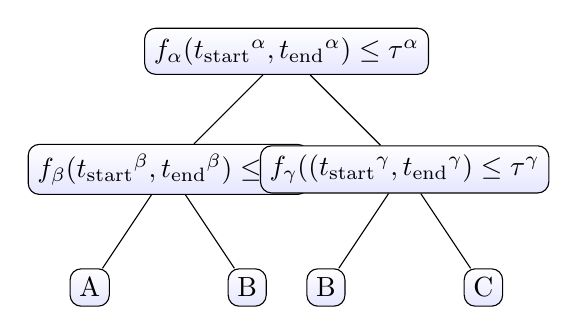
\begin{tikzpicture}[
    level 1/.style={sibling distance=30mm, level distance=15mm},
    level 2/.style={sibling distance=20mm, level distance=15mm},
    every node/.style = {shape=rectangle, rounded corners, draw, align=center, top color=white, bottom color=blue!10}
  ]
\node {\(f_{\alpha} ({t_{\mathrm{start}}}^{\alpha}, {t_{\mathrm{end}}}^\alpha) \leq \tau^{\alpha}\)}
  child {
    node {\(f_{\beta} ({t_{\mathrm{start}}}^{\beta}, {t_{\mathrm{end}}}^\beta) \leq \tau^{\beta}\)}
      child { node {A} }
      child { node {B} }
  }
  child {
    node {\(f_{\gamma} (({t_{\mathrm{start}}}^{\gamma}, {t_{\mathrm{end}}}^\gamma) \leq \tau^{\gamma}\)}
      child { node {B} }
      child { node {C} }
  };
\end{tikzpicture}

\subsubsection*{Random Forests}
To now classify a timeseries not just one tree is used. 
Multiple trees give their class prediciton, which is then 
aggregated and shown as a class probabilty. For this process to make sense
each tree should look at a diverse set of features. This is done by 
using a random sampling strategy in the training of each tree. 

The combination of many relatively uncorrelated trees can produce a forest whose prediction is more accurate than that of any of the individual trees. %% TODO: qutoe it from random forests
\subsection{Entropy and Entropy Gain}
Entropy gain is a widely used criterion to evaluate a split 
in a tree node. It quantifices the reduction in class impurity
after a given split. The higher the entropy gain, the better the 
seperation. 

Let $\{1, 2, ..., C\} := \mathfrak{C}$ be all class labels and 
$\gamma_c$ with $c \in \mathfrak{C}$ the proportion of the class $c$ in 
the current dataset. Then entropy is defined as 
\[
	\operatorname{Entropy}(\operatorname{data}) := - \sum_{c = 1}^{C} \gamma_c \log \gamma_c
\]
At a node the dataset is split into two and passed to the 
nodes children. Those new datasets have a different entropy than the 
parents dataset, with a lower entropy meaning a better purity. 
Let $\operatorname{ds}_{p}$ with $n_{p} = |\operatorname{ds}_p|$ be the parents dataset and $\operatorname{ds}_{l}, \operatorname{ds}_{r}$ with $n_{l}, n_{r} = |\operatorname{ds}_{l}|, |\operatorname{ds}_{r}|$ the childrens.
To now measure the entropy gain following formular is used.
\[
	\Delta \operatorname{Entropy} = \operatorname{Entropy}(\operatorname{ds}_p) - \left(\frac{n_{l}}{n_{p}}\operatorname{Entropy}(\operatorname{ds}_{l}) + \frac{n_{r}}{n_{p}} \operatorname{Entropy}(\operatorname{ds}_{r})\right)
\]
	

So lower entropy meaning higher purity in the children adjustet for the sizes of the datasets will lead to higher entropy gain.


\section{Time Series Forest Classifier (TSF)}
\subsection{Entrance Gain}
Entropy gain however has its limits, because "the number of  %TODO: ref Entropy gain
candidate splits can be large, and there are often cases 
where multiple candidate splits have the same $\Delta\operatorname{Entropy}$. %TODO: ref main paper


The paper introduced the splitting criterion entrance gain. % TODO: ref
For this the difference between the the threshold $\tau$ and the value
of the interval feature of all timeseries in the dataset is considered. The minimum
of all those values is called the $\operatorname{Margin}$.

For a split $f_k^n(t_{\mathrm{start}}, t_{\mathrm{end}}) \leq \tau$ for the timeseries $n$ 
\[
	\operatorname{Margin} = \min_{n = 1,2, ..., N} \left|f_k^n (t_{\mathrm{start}}, t_{\mathrm{end}}) - \tau \right|
\]

Entrance gain $E$ then is the combination of this Margin and $\Delta$Entropy with a a scalar $\alpha$ small 
enough to make the entrance gain a tiebreaker and nothing more.

\[
	E = \Delta\operatorname{Entropy} + \alpha \cdot\operatorname{Margin}
\]


\subsection{Main algorithm}
To build now a tree a recursive function is used. In each recursion step a single node of the 
tree is created. Each node holds an entrance gain $E^*$, an entropy gain $\Delta Entropy^*$, the 
interval $(t_{\mathrm{start}}, t_{\mathrm{end}})^*$, a threshold $\tau^*$ and an interval feature $f_*$.

\subsubsection*{Random Sampling Strategy}
The feature space of all possible intervals for a timeseries the length of $M$
is $O(M^2)$. To reduce this feature space an algorithm $SampleIntervals()$ is introduced. % TODO: ref algo
It first randomly samples $\sqrt{M}$ interval sizes. Then for each interval size $w$ it selects
a set of starting points from $\{1, \dots, M-w+1\}$. The size of the set is $\sqrt{M - w + 1}$, so that 
there are fewer starting points for larger interval sizes. For all these starting points $t_{start}$ the point 
$t_{end} = t_{start} + w - 1 $ is added to the set of all intervals, so that the feature space gets reduced to 
$O(\sqrt{M} \cdot \sqrt{M}) = O(M)$.

\begin{algorithm}[H]
\caption{\textsc{SampleIntervals}$(M)$, The function RandSampNoRep(set, samplesize)
randomly selects samplesize elements from set without replacement.}
\begin{algorithmic}[1]
\State $T_{start} \gets \emptyset$, $T_{end} \gets \emptyset$
\State $W \gets \textsc{RandSampNoRep}(\{1, \dots, M\}, \sqrt{M})$
\ForAll{$w \in W$}
    \State $S \gets \textsc{RandSampNoRep}(\{1, \dots, M - w + 1\}, \sqrt{M - w + 1})$
    \ForAll{$t_{start} \in S$}
        \State $T_{start} \gets T_{start} \cup \{t_{start}\}$
        \State $T_{end}  \gets T_{end}  \cup \{t_{start}  + w - 1\}$
    \EndFor
\EndFor
\State \Return $\langle T_{start}, T_{end} \rangle$
\end{algorithmic}
\end{algorithm}

\subsubsection*{Threshold Set Calculation}

To identify suitable split points for each feature type $f_k$, 
TSF constructs a fixed-size set of candidate thresholds. 
Let $f_k (t_{\mathrm{start}}, t_{\mathrm{end}})$ denote the $k$-th interval feature 
computed over 
the interval $(t_{\mathrm{start}}, t_{\mathrm{end}})$ for all training instances at 
the current node. Let $V = \{ f_k^{(i)} (t_{\mathrm{start}}, t_{\mathrm{end}}) \mid i = 1, \dots, N \}$ 
be the set of resulting feature values across all $N$ 
instances.

TSF then assigns a fixed number of $\kappa$ threshold per feature.
This is achieved by first computing the minimum and 
maximum values in $V$, denoted $a = \min V$ and 
$b = \max V$, respectively. The interval $[a, b]$ 
is then divided into $\kappa + 1$ equal-width segments.
The $\kappa$ internal division points are used as 
candidate thresholds:
\begin{equation*}
\tau_j = a + j \cdot \frac{b - a}{\kappa + 1}, \quad j = 1, 2, \dots, \kappa
\end{equation*}
This method ensures that the thresholds are uniformly 
spaced across the feature value range and that their 
number remains constant regardless of data distribution or 
sample size. 

\subsubsection*{Recursion and Termination}
After getting the interval set from the $SampleIntervals()$ algorithm and computing the threshold-set for each feature type,
TSF loops over every possible interval, every possible threshold and every possible interval feature.
It then calculates the entropy and entrance gain for each combination and maximizes the entrance gain and saves the split data.
Afterwards it checks if the entropy gain is zero. This is the termination condition for the recursion and the node
is marked as a leaf. Then the data is split according to the best features, interval and threshold and the 
function is called on the left and right dataset to build the children of the node.
\begin{algorithm}[H]
\caption{\textsc{BuildTSFTree}$(\mathcal{D})$}
\begin{algorithmic}[1]
\State $\langle T_1, T_2 \rangle \gets \textsc{SampleIntervals}(M)$
\State Compute candidate thresholds $\text{Threshold}_k$ for each feature type $k$
\State Initialize $E^* \gets 0$, $\Delta H^* \gets 0$, $t_1^* \gets 0$, $t_2^* \gets 0$, $\tau^* \gets 0$, $f^* \gets \emptyset$
\ForAll{$(t_{start}, t_{end}) \in \langle T_{start}, T_{end} \rangle$}
    \For{$k = 1$ to $K$}
        \ForAll{$\tau \in \text{Threshold}_k$}
            \State Compute $\Delta Entropy$ and $E$ for $f_k(t_{start}, t_{end}) \le \tau$
            \If{$E > E^*$}
                \State $E^* \gets E$, 
				\State $\Delta Entropy^* \gets \Delta Entropy$, 
				\State $t_{start}^* \gets t_{start}$, 
				\State $t_{end}^* \gets t_{end}$, 
				\State $\tau^* \gets \tau$, 
				\State $f^* \gets f_k$
            \EndIf
        \EndFor
    \EndFor
\EndFor
\If{$\Delta Entropy^* = 0$}
    \State \Return leaf node with majority class of $\mathcal{D}$
\EndIf
\State $\mathcal{D}_{\text{left}} \gets \{(X, y) \in \mathcal{D} \mid f^*(X[t_{start}^*:t_{end}^*]) \le \tau^* \}$
\State $\mathcal{D}_{\text{right}} \gets \{(X, y) \in \mathcal{D} \mid f^*(X[t_{start}^*:t_{end}^*]) > \tau^* \}$
\State node.left $\gets$ \Call{BuildTSFTree}{$\mathcal{D}_{\text{left}}$}
\State node.right $\gets$ \Call{BuildTSFTree}{$\mathcal{D}_{\text{right}}$}
\State \Return internal node with $(f^*, t_{start}^*, t_{end}^*, \tau^*, node.left, node.right)$
\end{algorithmic}
\end{algorithm}

\subsection{Complexity}
At each node running the for loops has a complexity 
of $M$ intervals, 3 interval features and $\kappa$ thresholds.
Each depth of the tree has at most $|data| = N$ nodes and the maximum depth of a tree can be assumed
as $O(\log N)$. As $\kappa$ is a constant the time complexity
for a single tree can be seen as $O(M N \log N)$. For a forest 
with $nTree$ trees that means the time complexity is at most $O(nTree M N \log N)$
\subsection{Temporal Importance Curve}
"TSF consists of multiple trees and is difficult to understand", so 
there is need for a method to extract interpretability from a 
forest. The temporal importance curve is introduced to reveal which parts of the 
time series contribute most to the classification decision. For that am importance function is built for each feature type and
used for all time points of the dataset. The Curve then is built by graphing those results out.

The importance function is based on the entropy gain of each split node $v$ in the forest $SN$ for the given feature type. All the 
nodes which intervals time-point $t$ are considered and their entropy gain for the given feature type is 
summed up. If the feature is not used in the split of the node, the entropy gain is set to zero.

\[
	\operatorname{Imp}_k(t) = \sum_{t_{start} \leq t \leq t_{end}, v \in SN}
\]

The method reveals temporal patterns in the data relevant for classification. Peaks in the curve indicate time regions used by strong splits.
Because points in the center of the series appear in more intervals, there is a natural bias towards them. To counteract this, the authors compare
uninformative datasets with the calculated importance curve. %TODO: ref dataset figure 

In practice, the curves highlight discriminative intervals successfully %TODO: ref 
As an example % TODO: ref
the temporal importance curves peak precisely in regions with specific intervals %TODO: figure

Using this method of observing the strength of the splits, it can be shown that entrance gain gives sharper and 
more localized peaks, thus improving the interpretability and specificity of the importance curves.

\section{Supervised Time Series
Forest (STSF)}
\subsection{Approach}
STSF uses a similar algorithm as TSF to build decision trees. 
However the difference lies in the feature space used, the time series representation 
and the sampling strategy. The goal is to reduce the interval space size 
to $O(\log M)$ and to find more discriminate intervals to achieve better classification.
Instead of relying on random intervals, it employs
a supervised search to identify informative intervals 
across multiple representations.
\subsection{Time Series Representations}

In TSF only the original/time-domain representation of a time series is looked at.
To capture a broader range of discriminations STSF uses multiple representations.
\subsubsection*{Periodogram}
Using a discrete Fourier transform the time series is mapped into the 
frequency domain. This allows STSF to detect intervals with discriminative periodic patterns,
even if they occur at varying time points across instances. "A side benefit of this 
representation is that it helps to indirectly detect phase-independent discriminatory intervals, i.e.m
discriminatory features located at different time regions of the original series as described in 
\Cref{fig:perio}" 

\begin{figure}[h]
\centering
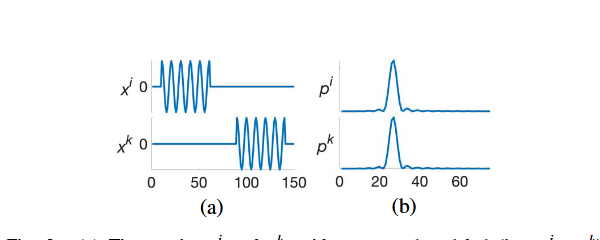
\includegraphics[width=\linewidth]{res/periobullshit.png}
\caption{"(a) Time series $x^i$ and $x^k$, with a same class label (i.e., $y^i = y^k$)
present a similar sub-series but located at different time regions (i.e., phase-
independent). (b) The periodogram representation $p^i$ and $p^k$ of series $x^i$ and
$x^k$, respectively. Our algorithm searches for discriminatory phase-dependent
interval features and cannot find discriminatory intervals that identify both
series as similar. The periodogram representation provides more flexibility
as it considers the frequency of the discriminatory sub-series (ignoring its
location in time) and thus helps to identify discriminatory sub-series even
when they appear at different locations in time across different time series."} % TODO: ref
\label{fig:perio}
\end{figure}
\subsubsection*{Derivative representation}
STSF also adopts the derivative representation as one of three complementary views 
on the input time series. The derivative captures local trends. This view emphasizes hte shape or dynamic behavior of the 
series over absolute levels. "The
discrete derivative of a time series $f$ with length $n$ is defined by
\[
	f'(i) = f(i) - f(i - 1) \forall ~ i \in \{2,3, \dots, n\}
\] %TODO: cite derivative


\subsection{Fisher Score}
To select a candidate feature there needs to be a ranking metric. 
Here the Fisher score is introduced. It is designed to indicate
the discriminatory effect of a feature. Let $y$ be 
the class label vector for $n$ timeseries $y \in \{1,2,\dots,c\}$ and 
$\alpha$ be an interval feature. Then let $\mu^{\alpha}$ be the overall mean of elements in $\alpha$ and $\mu^{\alpha}_k, \sigma^{\alpha}_k$ be the mean and standard
deviation of all the $k$-class elements in $\alpha$. 
The Fisher score is defined as :
\[
  \operatorname{FisherScore}(\alpha, y) = 
  \frac{\sum_{k = 1}^c n_k\left(\mu_k^{\alpha} - \mu^{\alpha}\right)^2}
       {\sum_{k = 1}^{c} n_k\left(\sigma_k^{\alpha}\right)^2}
\]
The Fisher score is chosen for its fast computation, but other metrics are also possible.
\subsection{Supervised Search}
The algorithm loops over all 3 representation and gives back samples denoted as 
$A_O, A_F$ and $A_D$ respectively.
All together then are used as the samples for the TSF algorithm $A^* = A_O \cup A_F \cup A_D$ %TODO: ref
Each Set $A_R$ is generated by recursively searching for class discriminative 
interval features across multiple random partitions of the input data.
Let $X \in \mathbb{R}^{n \times m}$ be the dataset of $n$ univariate time series of length
$m$ and let $y\in \{1, \dots, c\}^n$ be the vector for class labels.
For every interval feature $f_k$ %TODO: ref
the algorithm select a random split index $u\in \{1,\dots, m-1 \}$ to divide each time series into a 
left and right sub-series. $X_L\in \mathbb{R}^{n \times u}, X_R \in \mathbb{R}^{n \times (m - u)}$
This randomized partitioning is repeated a fixed number of times to increase diversity of the search space. 
For each representation and aggregation function, the algorithm then applies a recursive supervised function on both halves via
SupervisedSearch($X_L$, $f_k$, $y$, $f_r= \text{Fisher score}$, $A={}$) and SupervisedSearch($X_L$, $f_k$, $y$, $f_r = \text{Fisher score}$, $A={}$)

This function works as follows: it recursively bisects the interval, evaluates the two resulting sub-intervals using the aggregation function $f_k$, 
and scores the resulting feature vector with the ranking metric $f_r$.
The half with the higher score is retained in $A$ and further partitioned, while the other is discarded.
The termination of the function is when the interval length falls below 2.

Each path gives one interval feature, which is defined by its start and end indices and the function used. 
Since the loops are constant and the procedure follows a binary partitioning pattern,
it returns $O(\log m)$ features per call. These features are collected into $A_R$ and ultimately passed into the 
tree classifier, which selects final splits during training.


\begin{algorithm}[H]
\caption{SupervisedSearch}
\begin{algorithmic}[1]
\Require $X' \in \mathbb{R}^{n \times m'}$: time series set, $y \in \{1,\dots,c\}^n$: class labels,\\
\hspace{1.6em} $f$: aggregation function, $f_r$: feature ranking metric, $\bar{A}$: set of candidate intervals
\Ensure Updated set $\bar{A}$ of discriminatory interval features

\If{$m' < 2$}
    \State \Return $\bar{A}$
\Else
    \State $a_L \gets f(X', 1, m'/2)$
    \State $a_R \gets f(X', m'/2, m')$
    \State $score_L \gets f_r(a_L, y)$
    \State $score_R \gets f_r(a_R, y)$
    \If{$score_L \geq score_R$}
        \State $\bar{A} \gets \bar{A} \cup \{a_L\}$
        \State \Call{SupervisedSearch}{$X'[:, 1:m'/2]$, $y$, $f$, $f_r$, $\bar{A}$}
    \Else
        \State $\bar{A} \gets \bar{A} \cup \{a_R\}$
        \State \Call{SupervisedSearch}{$X'[:, m'/2:m']$, $y$, $f$, $f_r$, $\bar{A}$}
    \EndIf
\EndIf
\State \Return $\bar{A}$
\end{algorithmic}
\end{algorithm}

\subsection{Tree Construction}
To now construct trees a modified TSF is used. Instead 
of getting random samples the feature set is passed through the construction method.
Then as in TSF entrance gain is maximized. This approach has a faster complexity, because 
the sample size is reduced to $O(\log m)$, so that the
complexity drops to $O(nTree \log m N \log N)$, where $N$ is the maximum depth of the 
tree and $nTree$ is the amount of trees created. %TODO: ref complexity



\section{Experiments}
\subsection{Classification accuracy}
\subsubsection*{Setup}
STSF and TSF is tested on a set of 85 benchmark datesets. %TODO: ref the same
It is also compared to 1NN-DTW, RISE, BOSS, FCN, ResNet, Hive-Cote, PF and TS-CHIEF %TODO: ref
For every competitor the average classification accuracy is computed over 10 runs for each dataset.

\subsubsection*{Result}
As seen in Table \Cref{tab:stsf_full_results} STSF ranks higher on average than 1NN-DTW, TSF, RISE, PF, FCN and BOSS.
Only ResNet, HIVE-COTE, and TS-CHIEF rank higher than STSF. 
TSFs accuracy is the second lowest, only beating 1NN-DTW. 
Considering the trade offs in interpretability for TSF and speed for STSF however these results bode well for the two algorithms, because the 
difference in accuracy is so small. Through this test it has been shown that both can archieve state of the 
art accuracy.
\begin{table}[h]
\centering
\caption{Average classification accuracy and rank of all compared methods from the STSF benchmark}
\label{tab:stsf_full_results}
\begin{tabular}{lcc}
\toprule
\textbf{Method} & \textbf{Average Accuracy (\%)} & \textbf{Average Rank} \\
\midrule
1NN-DTW     & 75.91 & 8.16 \\
TSF         & 78.19 & 6.90 \\
RISE        & 78.84 & 6.55 \\
BOSS        & 81.16 & 6.10 \\
FCN         & 80.92 & 5.57 \\
ResNet      & 82.48 & 4.70 \\
HIVE-COTE   & 84.71 & 3.36 \\
PF          & 81.94 & 5.42 \\
TS-CHIEF    & 84.64 & 3.28 \\
STSF        & 82.60 & 4.95 \\
\bottomrule
\end{tabular}
\end{table}


\subsection{Training time}
\input{content/experiments/training.tex}
\section{Conclusion}
Time Series Forest (TSF) nad its successor, the Randomized-Supervised
Time Series Forest(r-STSF), show both complementary advances in classifying time series.
The goal is the same: Achieve interpretable, accurate classification in linear time complexity.
They manage to use simple changes to existing algorithms to built decision trees without resorting to overly
complex feature engineering. TSF introduces the core insight of using 
randomly sampled interval values with a custom splitting criterion, which outperforms
previous algorithms built on entropy gain. This simply adjustment enables TSF to 
outperform strong baselines like NN-DTW on a wide range of benchmarks, while preserving the 
key advantage of interpretability via temporal importance curves.

The reliance on purely random feature generation, limits TSF in settings where the 
relevant temporal structure is sparse or subtle %TODO: ref
Precision is sacrificed for robustness %ref TODO:
Also while being conceptually elegant, the temporal importance curve 
is biased toward central indices due to interval frequency effects. TSF does not introduce 
a mechanism for normalizing or filtering out these uninformative peaks.

These issues are addressed in the construction of STSF, by replacing node-level feature randomness
with tree-level interval supervision. A pre-search of the entire time series using a Fisher score-based strategy
is used to identify candidate discriminatory intervals
It also further enhances coverage with 
through multiple time series representation.
These mechanisms increase both precision and efficiency resulting in STSF achieving better accuracy than TSF while being an 
order of magnitude faster on long series. %TODO: ref

Despite these improvements, STSF comes with new costs: 
interpretability suffers and especially t
%TODO: REF DESPERATLY NEEDED

In sum, TSF and STSF show that it is possible to build time series classifiers that combine
competitiveness with interpretability. TSF leverages randomness to ensure robustness and simplicity and 
r-STSF introduces supervision to increase focus and precision. They establish a foundation for interval-based 
methods that are both practical and transparent. Their success suggests that refining how and where
information is extracted within the time series is preferable to increasing
complexity.

\section{Literature}
You should have 10 citations from peer reviewed papers and/or books. \\
Length estimate: 1/2 column

\end{document}